\documentclass[autodetect-engine,dvipdfmx-if-dvi,ja=standard]{bxjsarticle}

% 二段組にするとき
% \documentclass[twocolumn,autodetect-engine,dvipdfmx-if-dvi,ja=standard]{bxjsarticle}

\usepackage{graphicx}        %図を表示するのに必要
\usepackage{color}           %jpgなどを表示するのに必要
\usepackage{amsmath,amssymb} %数学記号を出すのに必要
\usepackage{setspace}
\usepackage{eclclass}
\usepackage{cases}
\usepackage{here}
\usepackage{fancyhdr}
\usepackage{ascmac}

% 文書全体のスタイルを設定(主に余白)
\setlength{\topmargin}{-0.3in}
\setlength{\oddsidemargin}{0pt}
\setlength{\evensidemargin}{0pt}
\setlength{\textheight}{44\baselineskip}

% 行頭の字下げをしない
\parindent = 0pt

% ヘッダとフッタの設定
\lhead{電気情報工学応用実験II}
\chead{}
\rhead{5E 20番 佐藤凌雅}
\lfoot{}
\cfoot{-\thepage-} % ページ数
\rfoot{}

% 式の番号を(senction_num.num)のようにする
\makeatletter
\@addtoreset{equation}{section}
\def\theequation{\thesection.\arabic{equation}}
\makeatother

% 画像の貼り付けを簡単にする
\newcommand{\pic}[2]
{
  \begin{figure}[H]
    \begin{center}
      \includegraphics[scale=#2]{#1}
    \end{center}
  \end{figure}
}

% 単位の記述を簡単にする
\newcommand{\unit}[1]
{
  \, [\mathrm{#1}]
}
% \title{一次元物質の評価 \\ 一次元物質の数値計算による電子状態および物性評価}
% \date{\today}
\begin{document}
% \maketitle
\pagestyle{fancy}

\section{目的}
 次のことを数値的に検証することを目的とする.
\begin{enumerate}
  \item フェルミエネルギーがバンドギャップの中にある時に絶縁体(半導体)となること,及び,ギャップの外にある時に導体になること.
  \item バンドギャップの中の電子状態密度がゼロ(外がノンゼロ)になること.
  \item 一次元物質の場合,電子状態密度が,エネルギー分散の傾きに反比例すること.
\end{enumerate}

\section{実験概要}
 グラフェンナノリボン(GNR)の電子状態を,強束縛(タイトバインディング)近似法に基づいて求める.その際,炭素原子の$2p_z$軌道にのみを扱い,他の軌道は無視する.さらに,エネルギー分散,電子状態密度(DOS),電気伝導度(コンダクタンス),及び電流分布を求める.以上の全てを数値計算で求める.

\section{理論}
\subsection{グラフェンナノリボン(GNR)}
 グラフェンとは,炭素原子が蜂の巣状に並んだ二次元シート状物質のこと.GNRとは,その一部を切り取って出来る一次元ワイヤー状物質のこと.GNRの電子状態は,グラフェンの切り取り方に依存して変化するため,電気伝導特性も切り取り方に依存する.\\

 ここでは,アームチェア型のGNRを使用する.アームチェア型の GNR とは,図1\footnote{カーボンナノチューブの構造,http://www.center.shizuoka-c.ed.jp/,2019-4-11閲覧}のように,ワイヤー断面の両端(エッジ)がアームチェアの形をしている GNR のことである.アームチェア型GNRは,ワイヤー幅に依存して,絶縁体(半導体)になったり,導体になったりすることが知られている.

\begin{figure}[H]
  \centering
  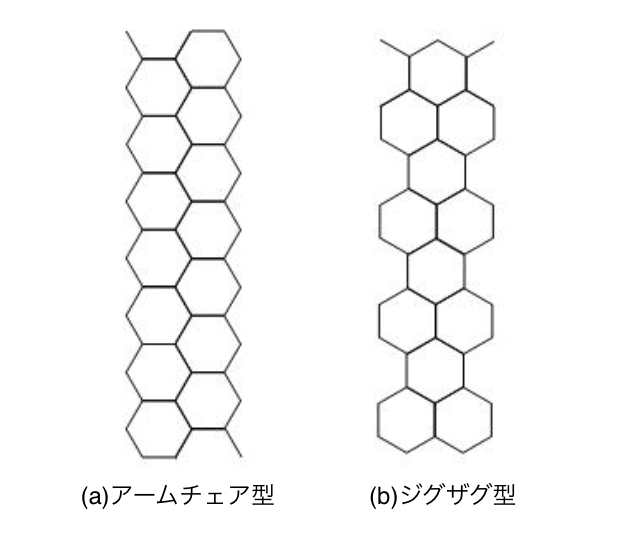
\includegraphics[height=5cm]{./imgs/1.png}
  \caption{グラフェン・ナノリボンの構造:アームチェアとジグザグ}
\end{figure}

\subsection{GNRの電子状態}
 GNRは二次元シート状のグラフェンを切り取って出来る一次元ワイヤーである.エネルギー分散$E\left(k\right)$は,次のようになる.

\begin{flalign}
&E\left(k\right) = \pm \sqrt{1+4\cos\left(\dfrac{n}{N+1}\pi\right) \cos\left(\dfrac{k}{2}\right)+4\cos^2\left(\dfrac{n}{N+1}\pi\right)}
\end{flalign}

 ただし,$N$は,ワイヤーに平行で,なおかつ炭素原子上を通る直線の本数である.すなわち,ワイヤー幅はNに比例する.

\begin{figure}[H]
  \centering
  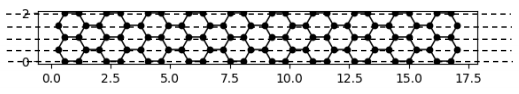
\includegraphics[width=10cm]{./imgs/2.png}
  \caption{グラフェン・ナノリボンの構造:アームチェアとジグザグ}
\end{figure}

 N=5に対する$E(k)$を図示すると,図3が得られる.これは,グラフェンのエネルギーのグラフにおいて,縦軸(//E)に平行で等間隔な平面の集合によってE(k)を切断したときに,それらの断面上に生じる曲線の集合である.その様子を図4に示す.

\begin{figure}[H]
  \centering

  \begin{tabular}{c}
    \begin{minipage}{0.50\hsize}
    \centering
    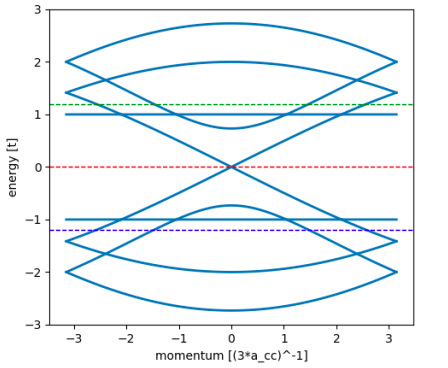
\includegraphics[keepaspectratio, height=5cm]{./imgs/3.png}
    \caption{$N= 5$に対する$E(k)$}
    \end{minipage}

    \begin{minipage}{0.50\hsize}
    \centering
    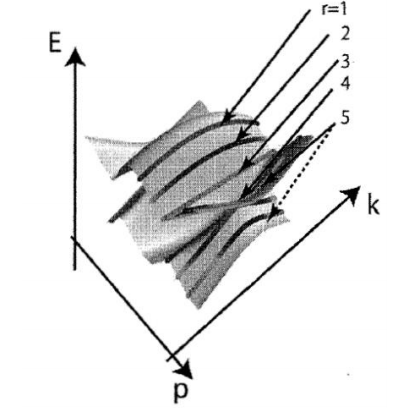
\includegraphics[keepaspectratio, height=5cm]{./imgs/4.png}
    \caption{グラフェンとGNRのエネルギーバンドの関係}
    \end{minipage}
  \end{tabular}
\end{figure}

 もし切断平面集合の中に,K点やK’点を通る平面が含まれている場合は,バンドギャップが形成されない.一方,集合内に,K 点やK’点を通る平面が存在しない場合は,バンドギャップが形成される.

\section{実験方法}
 図5のような4種類の太さのGNRを作成し,それらのエネルギー分散,電子状態密度(DOS),電気伝導度(コンダクタンス),および電流分布を求める.\\
 計算には,タイトバインディング計算用のpythonライブラリ「KWANT」を使用して記述されたソースコードを使用する.ソースコード,および計算環境は,担当教員によって,あらかじめ用意されている.
\begin{figure}[H]
  \centering
  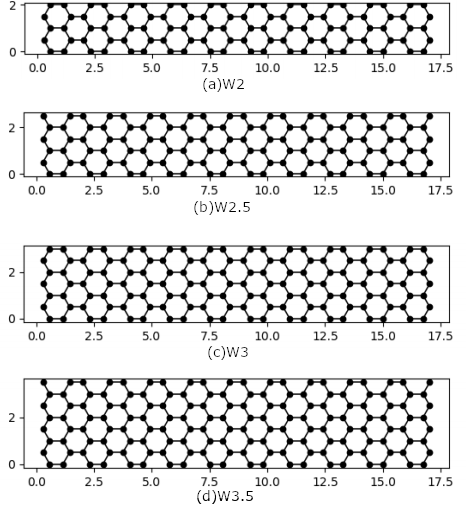
\includegraphics[width=7cm]{./imgs/5.png}
  \caption{GNRの結晶構造}
\end{figure}

\section{考察の方針}
 4種類のGNRのエネルギー分散,電子状態密度(DOS),電気伝導度(コンダクタンス),および電流分布を比較し,以下の検証を中心に考察する.
\begin{enumerate}
  \item フェルミエネルギーがバンドギャップの中にある時に絶縁体(半導体)となること,及び,ギャップの外にある時に導体になること.
  \item バンドギャップの中の電子状態密度がゼロ(外がノンゼロ)になること.
  \item 一次元物質の場合,電子状態密度が,エネルギー分散の傾きに反比例すること.
\end{enumerate}

 さらに,エネルギー分散の傾きがゼロのところで DOS が発散している理由や,コンダクタンスがステップ構造をとる理由について考察して正しい結論を導く.


\newpage

\section{実験結果}
\subsection{エネルギー分散}
 4種類(w=2.0,w=2.5,w=3.0,w=3.5)のGNRのエネルギー分散をそれぞれ図\ref{E:w=2.0}から図\ref{E:w=3.5}に示す.\\
\\
\begin{figure}[htpb]
  \centering

  \begin{tabular}{c}
    \begin{minipage}{0.50\hsize}
    \centering
    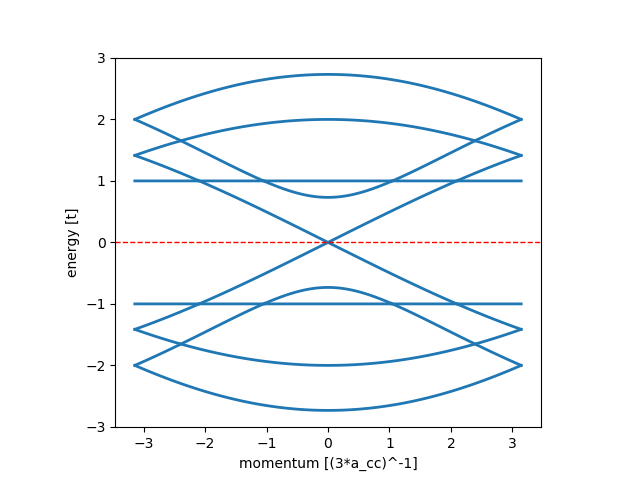
\includegraphics[keepaspectratio, scale=0.55]{./data/w2/w2-band_2.png}
    \caption{w=2.0のエネルギー分散}
    \label{E:w=2.0}
    \end{minipage}

    \begin{minipage}{0.50\hsize}
    \centering
    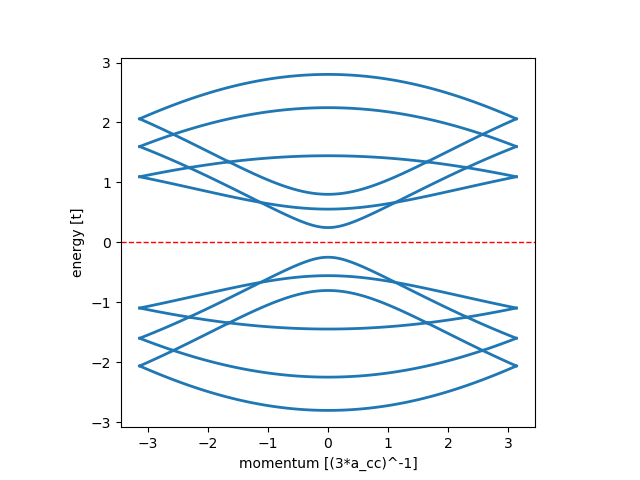
\includegraphics[keepaspectratio, scale=0.55]{./data/w2_5/w2_5-band_2.png}
    \caption{w=2.5のエネルギー分散}
    \end{minipage}

    \\
    \\

    \begin{minipage}{0.50\hsize}
    \centering
    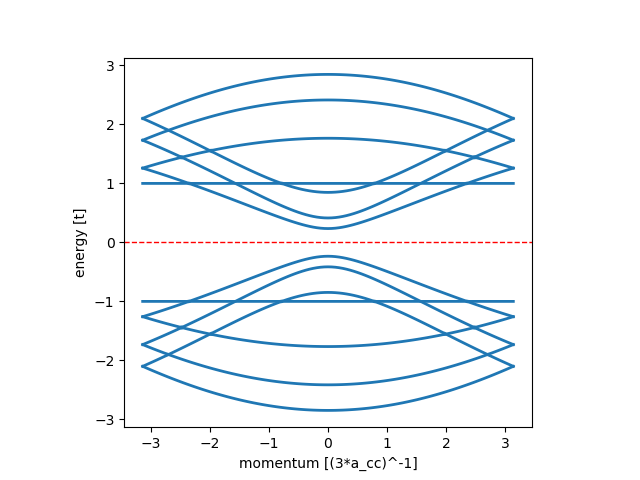
\includegraphics[keepaspectratio, scale=0.55]{./data/w3/w3-band_2.png}
    \caption{w=3.0のエネルギー分散}
    \end{minipage}

    \begin{minipage}{0.50\hsize}
    \centering
    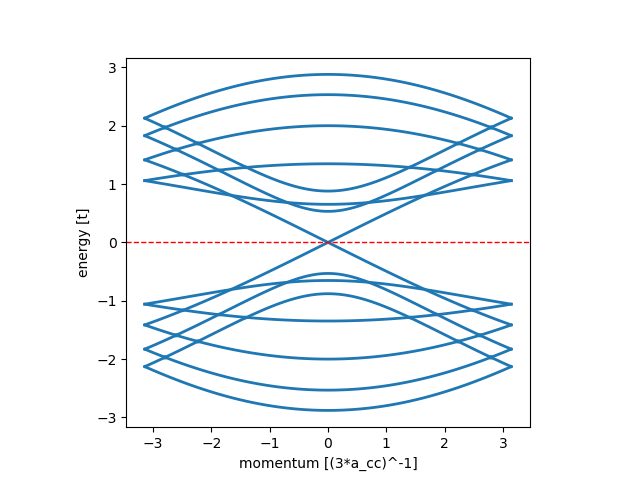
\includegraphics[keepaspectratio, scale=0.55]{./data/w3_5/w3_5-band_2.png}
    \caption{w=3.5のエネルギー分散}
    \label{E:w=3.5}
    \end{minipage}
  \end{tabular}
\end{figure}

\newpage
\subsection{電子状態密度(DOS)}
 4種類(w=2.0,w=2.5,w=3.0,w=3.5)の電子状態密度(DOS)をそれぞれ図\ref{DOS:w=2.0}から図\ref{DOS:w=3.5}に示す.\\
\\
\begin{figure}[htpb]
  \centering

  \begin{tabular}{c}
    \begin{minipage}{0.50\hsize}
    \centering
    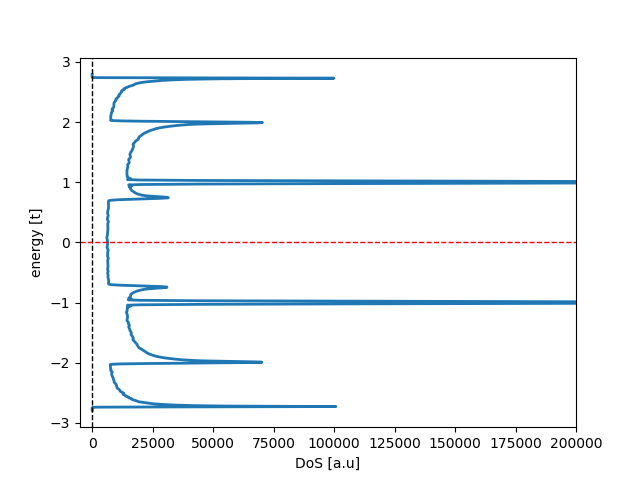
\includegraphics[keepaspectratio, scale=0.55]{./data/w2/w2-dos.png}
    \caption{w=2.0の電子状態密度}
    \label{DOS:w=2.0}
    \end{minipage}

    \begin{minipage}{0.50\hsize}
    \centering
    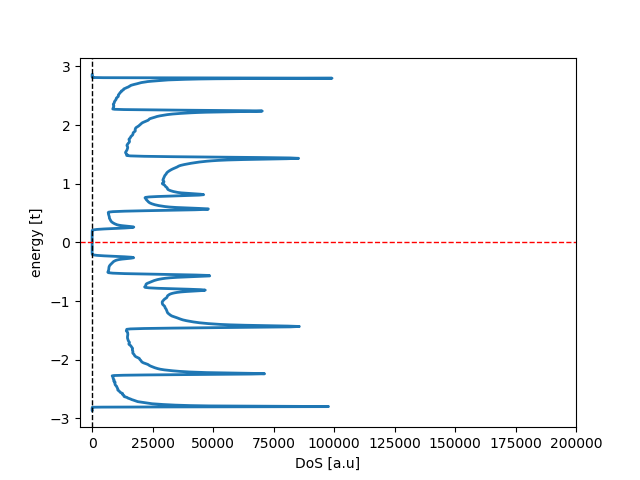
\includegraphics[keepaspectratio, scale=0.55]{./data/w2_5/w2_5-dos.png}
    \caption{w=2.5の電子状態密度}
    \end{minipage}

    \\
    \\

    \begin{minipage}{0.50\hsize}
    \centering
    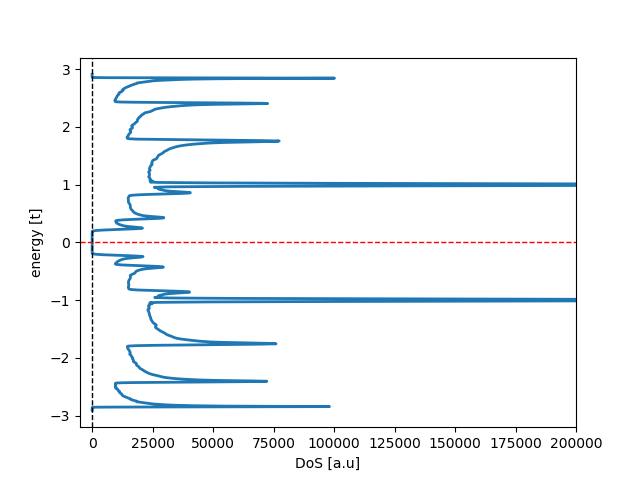
\includegraphics[keepaspectratio, scale=0.55]{./data/w3/w3-dos.png}
    \caption{w=3.0の電子状態密度}
    \end{minipage}

    \begin{minipage}{0.50\hsize}
    \centering
    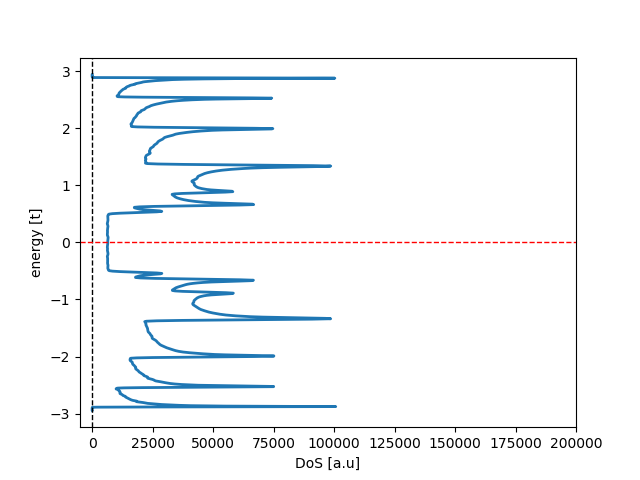
\includegraphics[keepaspectratio, scale=0.55]{./data/w3_5/w3_5-dos.png}
    \caption{w=3.5の電子状態密度}
    \label{DOS:w=3.5}
    \end{minipage}
  \end{tabular}
\end{figure}

\newpage
\subsection{コンダクタンス}
 4種類(w=2.0,w=2.5,w=3.0,w=3.5)のコンダクタンスをそれぞれ図\ref{cond:w=2.0}から図\ref{cond:w=3.5}に示す.\\
\\
\begin{figure}[htpb]
  \centering

  \begin{tabular}{c}
    \begin{minipage}{0.50\hsize}
    \centering
    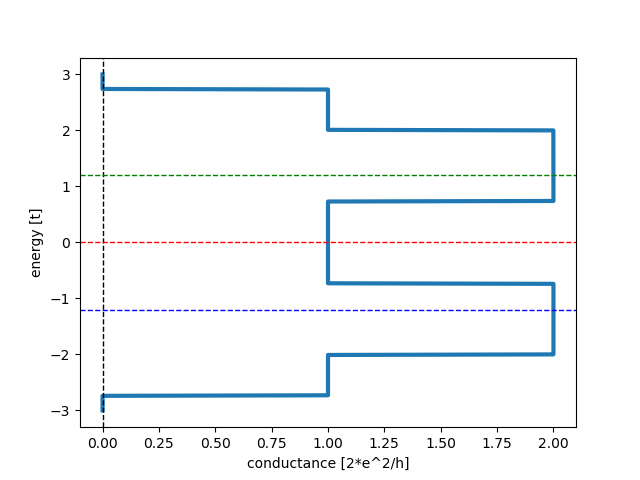
\includegraphics[keepaspectratio, scale=0.55]{./data/w2/w2-j_cond.png}
    \caption{w=2.0のコンダクタンス}
    \label{cond:w=2.0}
    \end{minipage}

    \begin{minipage}{0.50\hsize}
    \centering
    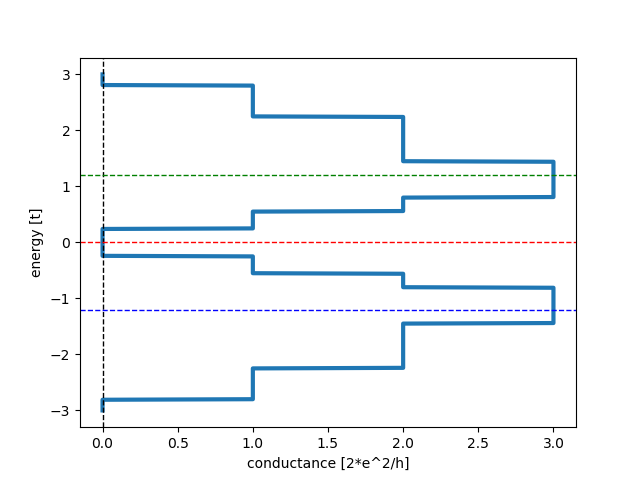
\includegraphics[keepaspectratio, scale=0.55]{./data/w2_5/w2_5-j_cond.png}
    \caption{w=2.5のコンダクタンス}
    \end{minipage}

    \\
    \\

    \begin{minipage}{0.50\hsize}
    \centering
    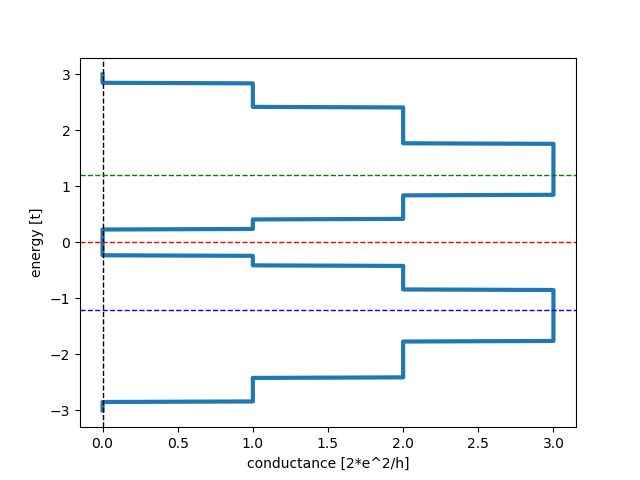
\includegraphics[keepaspectratio, scale=0.55]{./data/w3/w3-j_cond.png}
    \caption{w=3.0のコンダクタンス}
    \end{minipage}

    \begin{minipage}{0.50\hsize}
    \centering
    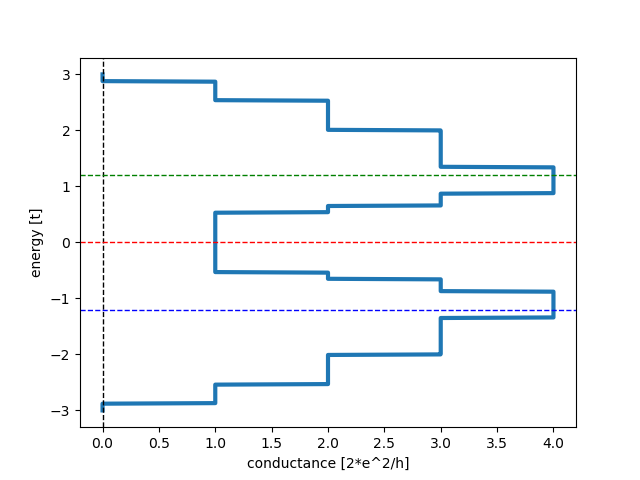
\includegraphics[keepaspectratio, scale=0.55]{./data/w3_5/w3_5-j_cond.png}
    \caption{w=3.5のコンダクタンス}
    \label{cond:w=3.5}
    \end{minipage}
  \end{tabular}
\end{figure}

\newpage
\subsection{電流分布}
 w=2.0のGNRでエネルギーが-1.2,1.2,0における(図\ref{cond:w=2.0}での青,緑,赤に対応する)電流分布をそれぞれ図\ref{j:m},図\ref{j:p},図\ref{j:z}に示す.\\
\\
\begin{figure}[htpb]
  \centering

  \begin{tabular}{c}
    \begin{minipage}{0.50\hsize}
    \centering
    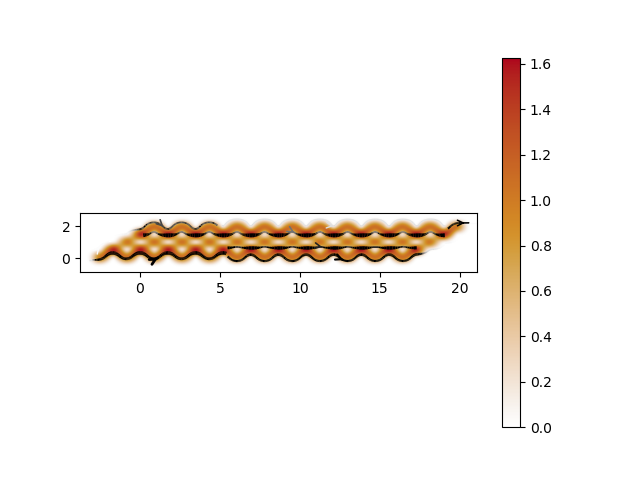
\includegraphics[keepaspectratio, scale=0.55]{./data/w2/w2-j_m1_2.png}
    \caption{エネルギーが-1.2での電流分布}
    \label{j:m}
    \end{minipage}

    \begin{minipage}{0.50\hsize}
    \centering
    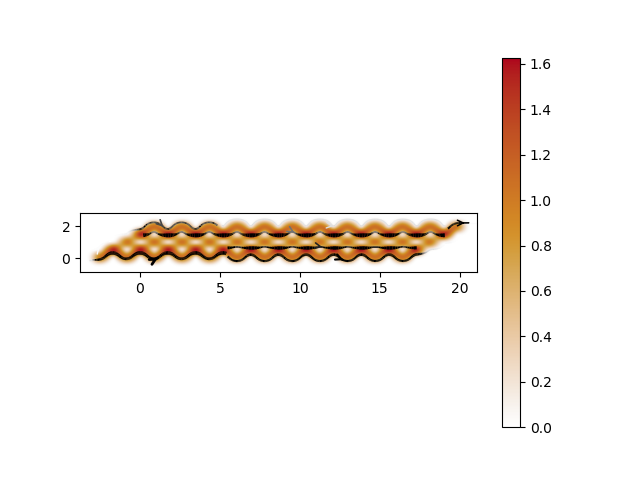
\includegraphics[keepaspectratio, scale=0.55]{./data/w2/w2-j_p1_2.png}
    \caption{エネルギーが1.2での電流分布}
    \label{j:p}
    \end{minipage}

    \\
    \\

    \begin{minipage}{0.50\hsize}
    \centering
    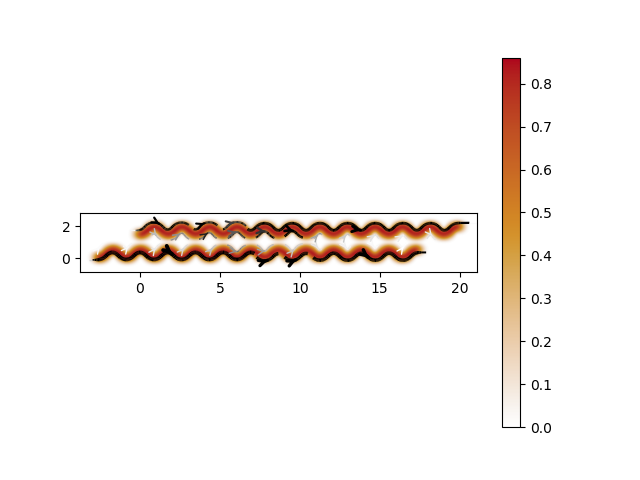
\includegraphics[keepaspectratio, scale=0.55]{./data/w2/w2-j_zero.png}
    \caption{エネルギーが0での電流分布}
    \label{j:z}
    \end{minipage}
  \end{tabular}
\end{figure}


\newpage

\section{考察}
 図6,図9のw=2.0,w=3.5でのエネルギー分散を見るとギャップが無く,図7,図8のw=2.5,w=3.0のエネルギー分散を見ると,ギャップがあることが確認できる.この時,w=2.0,w=3.5のコンダクタンス(図14,図17)を確認すると0でない値を取っていることがわかる.一方で,w=2.5,w=3.0のコンダクタンス(図15,図16)はゼロを取っており,不導体の性質を示していることが確認できる.\\
 以上のことから,フェルミエネルギーがバンドギャップの中にある時に不導体となり,ギャップの外にある時に導体になることが確認できた.\\

 w=2.0,w=3.5の電子状態密度(DOS)(図10,図13)はエネルギー0の際にノンゼロであった.一方,w=2.5,w=3.0のDOS(図11,図12)はエネルギー0の際に0となっていた.前述のように,図6〜図9のグラフから,w=2.0,w=3.5ではエネルギー0の際にギャップが存在せず,w=2.5,w=3.0の際にはギャップが確認されている.\\
 以上のことから,バンドギャップの内ではDOSはゼロとなることがわかる.\\

 エネルギー分散のグラフ(図6〜図9)とDOSのグラフ(図10〜図13)を比較すると,エネルギー分散の傾きが大きいポイントでは,DOSの値は小さくなっていることがわかる.加えて,エネルギー分散の傾きが0の点(図6のエネルギー1付近)ではDOSは発散している(図10のエネルギー1付近).\\
 このことから,エネルギー分散の傾きとDOSは反比例関係にあることが確認できる.\\

 今回のようなk空間で状態が等間隔に存在しているとき,空間でのDOS,すなわち単位波数当たりの状態密度は一定値$1/(\Delta k)$である.\\
 分散関係E(k)が単調であれば,E空間でのDOSは\\
\begin{flalign}
  &\rho(E)dE=\dfrac{dk}{\Delta k}
\end{flalign}
 より,\\
\begin{flalign}
  &\rho(E)=\dfrac{1}{\Delta k}\dfrac{\partial k}{\partial E}
\end{flalign}
 である.\\
 したがって,上のように$\dfrac{dE}{dk}=0$となる点においては,DOS状態密度は発散する.\\

 また,w2.5のエネルギー分散のグラフ(図7)を確認すると,エネルギーが-3から-2.8程度の間には交点は存在せず,-2.8から-2程度の間には2点,-1付近では6点の交点が存在している.一方で,w2.5のコンダクタンスのグラフ(図15)を見ると,エネルギーが-3から-2.8程度の間のコンダクタンスは1となっていた.-2付近は2,-1付近では3というコンダクタンスの値が出ていた.\\
 以上のことから,コンダクタンスの値は,エネルギー分散のグラフの交点と対応関係にあることがわかる.\\

\end{document}
